\section{Introduction}

Researcher mobility connects scientific communities across national borders and between cities within countries, facilitating knowledge exchange and collaboration \cite{ref006,ref029}. Discussions of brain drain and brain gain reflect broader concerns about the geographic distribution of researchers \cite{ref041,ref034}. The two spatial scales reveal different aspects of mobility. International flows connect national research systems, whereas domestic intercity flows trace movements among cities within those systems. As more countries and cities participate in researcher mobility, its geographic coverage may expand without a corresponding reduction in the concentration of flows. This distinction matters because the relative shares of incoming and outgoing flows indicate which countries and cities occupy more prominent positions in researcher mobility, with potential implications for the geography of scientific exchange. A central question is therefore how the expanding geography of researcher mobility relates to changes in its distribution across countries and cities, and whether these changes differ between international and domestic mobility.

\begin{figure}[!tbp]
\centering
\IfFileExists{figures/Fig1.pdf}{%
  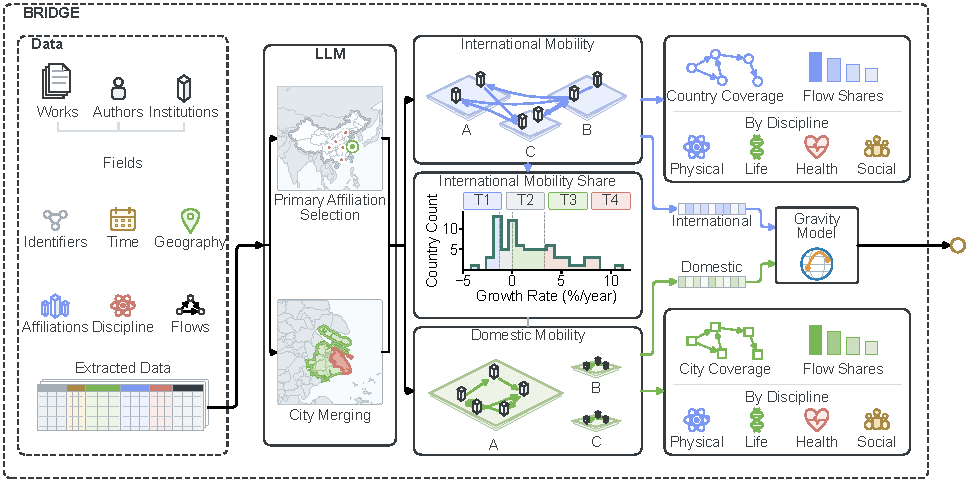
\includegraphics[width=\linewidth]{figures/Fig1.pdf}%
}{\IfFileExists{figures/Fig1.svg}{%
  \includesvg[inkscapelatex=false,width=\linewidth]{figures/Fig1}%
}{%
  \fbox{\parbox[c][32mm][c]{0.88\textwidth}{\centering\small
  Figure 1 artwork is missing.\\[4pt]
  Add \texttt{figures/Fig1.pdf} or \texttt{figures/Fig1.svg}.}}%
}}
\caption{\textbar\ \textbf{The BRIDGE Framework.} BRIDGE integrates linked publication, author and institution records with primary-affiliation selection and LLM-assisted city merging to support international and domestic mobility analyses. The histogram groups countries by fitted international-share growth: declining and rising shares are each split at their median (T1--T4, from faster decline to faster growth). Each scale compares coverage, flow shares and four disciplinary domains. International and domestic feature vectors include disciplinary information and enter the gravity model; the terminal circle denotes reconstructed domestic flows. In the maps, green denotes selected or harmonized cities; red denotes alternative affiliation cities or merged districts.}
\label{fig:fig1}
\end{figure}

Previous research has examined two related aspects of researcher mobility: changes in its geographic reach and direction, and differences in how mobility is distributed among places. At the international scale, the countries involved in cross-border movements have become increasingly diverse \cite{ref008}, while these movements have also exhibited growing regionalization \cite{ref038}. At the city level, studies of researcher mobility networks have identified highly connected urban centres \cite{ref026}, with highly productive researchers tending to move to and remain in globally central cities \cite{ref031}. Research examining international and internal mobility together has further revealed disparities in subnational migration rates and differences in regional mobility trajectories \cite{ref029,ref030}. Together, these studies provide complementary perspectives on the geographic reach of researcher mobility and the uneven distribution of movements across locations and spatial scales.

These studies establish that researcher mobility has reached more places\cite{ref008} and that flows and migration rates differ across places\cite{ref031,ref029}. How participation shapes changes in the distribution of flows remains less clear. As international mobility becomes more geographically dispersed, how widely are increases in global shares distributed across countries? Within countries, how does including newly recorded cities alter the measured distribution compared with following the same cities over time? Comparing these changes across disciplines can establish how consistently the international and domestic patterns occur and where the contrast is strongest.

To address these questions, we develop the Bilateral Relations in the Dynamics of Global Expansion (BRIDGE) analytical framework (Fig.~\ref{fig:fig1}). BRIDGE integrates publication, author and affiliation records with external geographic reference information, using large language model (LLM)-assisted city resolution to harmonize geographic locations across years. The framework examines two complementary dimensions of researcher mobility: geographic coverage, which captures participating countries, cities and their connections, and flow distribution, which describes how incoming and outgoing movements are distributed among locations. Together, these dimensions enable consistent longitudinal comparisons of international country-to-country and domestic intercity mobility. At the city level, BRIDGE distinguishes newly recorded cities from continuously recorded cities to assess their contributions to changes in geographic coverage and flow distribution. Disciplinary comparisons further examine whether these patterns are shared across fields. BRIDGE also incorporates gravity-based spatial-interaction modelling to examine how geographic, research-related and network factors, including international mobility connections, relate to mobility flow allocation \cite{lenormand2016}.

We analyse approximately 30 million researcher mobility events identified from author--affiliation records spanning 1998--2025. Annual directed networks capture international country-to-country and domestic intercity flows, together with the participating locations and connections. The main domestic intercity analysis includes 76 countries. Disciplinary comparisons span 26 fields grouped into four broad domains and use a matched sample of 45 countries. These data enable longitudinal comparisons of geographic coverage and flow distribution across spatial scales and scientific disciplines.

International flows became more evenly distributed across countries, while most of the increase in national shares accrued to a small subset of countries. Within countries, newly recorded cities carrying little flow contributed to rising concentration, while flows often became more even among continuously recorded cities. The cross-scale contrast appeared across all four disciplinary domains and was strongest in social sciences. In the matched disciplinary sample, the median domestic inequality trend reversed in every domain when the same cities were followed across years. Comparing the changing distribution with the distribution among persistent participants thus helps explain how mobility can reach more places while geographic disparities change in different directions.

\FloatBarrier
